\documentclass[aspectratio=169]{beamer}

% --------------------
% Theme (clean + academic)
% --------------------
\usetheme{Madrid}
\usecolortheme{default}
\setbeamertemplate{navigation symbols}{}

% --------------------
% Make Madrid look slimmer
% --------------------
\setbeamertemplate{navigation symbols}{}
\setbeamertemplate{blocks}[default] % no rounded/shadow boxes

% Remove colored block backgrounds (major visual simplification)
\setbeamercolor{block title}{fg=black,bg=white}
\setbeamercolor{block body}{fg=black,bg=white}
\setbeamercolor{block title alerted}{fg=black,bg=white}
\setbeamercolor{block body alerted}{fg=black,bg=white}

% Remove extra vertical space in blocks
\setlength{\abovedisplayskip}{6pt}
\setlength{\belowdisplayskip}{6pt}
\setlength{\abovedisplayshortskip}{4pt}
\setlength{\belowdisplayshortskip}{4pt}

% Slightly denser lists (but still readable)
\setlength{\itemsep}{3pt}
\setlength{\parskip}{2pt}
\setlength{\parsep}{0pt}

% Less distracting title bar
\setbeamercolor{frametitle}{fg=black,bg=white}
\setbeamertemplate{frametitle}{
  \vspace{0.2em}
  \insertframetitle
  \par\vspace{0.2em}\hrule
}


% --------------------
% Packages
% --------------------
\usepackage{amsmath, amssymb, amsfonts}
\usepackage{mathtools}
\usepackage{bm}

% --------------------
% Shortcuts
% --------------------
\newcommand{\Om}{\Omega}
\newcommand{\M}{\mathcal{M}}
\newcommand{\Cz}{C_0(\Om)}
\newcommand{\ip}[2]{\left\langle #1,#2\right\rangle}
\newcommand{\norm}[1]{\left\lVert #1\right\rVert}
\newcommand{\supp}{\operatorname{supp}}

% --------------------
% Title info
% --------------------
\title[Elliptic Control with Measures]{Elliptic Optimal Control with Measure-Valued Controls}
\subtitle{Predual reformulation, sparsity, and semismooth Newton numerics}
\author{Anderson Singulani}
\institute{Seminar}
\date{January 21, 2026}

\begin{document}

% ============================================================
% TITLE
% ============================================================
\begin{frame}
  \titlepage
\end{frame}

% ============================================================
% ROADMAP
% ============================================================
\begin{frame}{Roadmap}
\begin{itemize}
  \item Motivation: localized actuation and sparsity
  \item Setup PDE with measure data
  \item Optimization problem 
  \item Optimality conditions and sparsity structure 
  \item Numerics and regularization
  \item Experiments
  \item Conclusion
\end{itemize}
\end{frame}

% ============================================================
% MOTIVATION
% ============================================================
\begin{frame}{Motivation: why measure-valued controls?}

Desired properties 
\begin{itemize}
  \item \textbf{Localized actuation:} heating spots, micro-heaters, point electrodes, concentrated loads.
  \item \textbf{Natural model:} point sources $\approx$ Dirac measures $\Rightarrow u\in\mathcal M(\Omega)$.
  \item \textbf{Sparsity:} $L^1$-type penalties promote concentrated/active-set solutions.
\end{itemize}

\medskip
\textbf{Main challenge:} nonsmooth cost in a nonreflexive space.
\end{frame}

% ============================================================
% PDE WITH MEASURE DATA
% ============================================================
\begin{frame}{Setup | Elliptic PDE with measure data}
We consider
\[
Ay = u \quad \text{in }\Om,\qquad y=0 \quad\text{on }\partial\Om,
\qquad u\in \M(\Om).
\]

\begin{block}{Why not the usual $H^1_0$ formulation?}
A general measure $u$ is \emph{not} in $H^{-1}(\Om)$, so
testing with $v\in H^1_0(\Om)$ is not well-defined.
\end{block}

\begin{block}{Very weak formulation (Dirichlet)}
Choose a test space $V \hookrightarrow C_0(\Om)$, e.g.
$V = H^2(\Om)\cap H^1_0(\Om)$ (in $n=2,3$).
Then there exist $y\in L^1(\Om)$ that solves
\[
\int_\Om y\, A^\ast \varphi\, dx = \int_\Om \varphi\, du
\qquad \forall \varphi\in V.
\]
\end{block}
\end{frame}

% ============================================================
% REGULARITY / SOLUTION OPERATOR
% ============================================================
\begin{frame}{Setup | Regularity and the solution map}
\begin{block}{Elliptic smoothing for measure data}
For $u\in \M(\Om)$, the very weak solution satisfies
\[
y \in W^{1,p}_0(\Om)\quad \text{for all } 1\le p < \frac{n}{n-1},
\qquad
\norm{y}_{W^{1,p}} \le C \norm{u}_{\M(\Om)}.
\]
\end{block}

\begin{block}{Solution operator}
Define
\[
S:\M(\Om)\to L^2(\Om),\qquad Su = y(u),
\]
using Sobolev embedding $W^{1,p}_0(\Om)\hookrightarrow L^2(\Om)$ (for suitable $p$, $n\in\{2,3\}$).
\end{block}

\begin{alertblock}{Key takeaway}
Even if $u$ is singular (Dirac), the state $y$ is a genuine function usable in an $L^2$ tracking term.
\end{alertblock}
\end{frame}

% ============================================================
% PRIMAL PROBLEM
% ============================================================
\begin{frame}{Optimization problem | Primal sparse control problem in $\M(\Om)$}
Given desired state $z\in L^2(\Om)$ and $\alpha>0$:
\[
\min_{u\in \M(\Om)}\;
J(u):=\frac12 \norm{Su-z}_{L^2(\Om)}^2 + \alpha \norm{u}_{\M(\Om)}.
\]

\begin{block}{Interpretation}
\begin{itemize}
  \item $\frac12\norm{Su-z}^2$: match the target state
  \item $\alpha\norm{u}_{\M}$: pay for total control mass $\Rightarrow$ sparse actuation
\end{itemize}
\end{block}

\begin{alertblock}{Two difficulties}
\begin{itemize}
  \item Nonsmooth term $\norm{u}_\M$
  \item Nonreflexive space $\M(\Om)$
\end{itemize}
\end{alertblock}
\end{frame}

% ============================================================
% EXISTENCE / UNIQUENESS
% ============================================================
%\begin{frame}{Optimization problem | Existence and uniqueness (direct method)}
%\begin{block}{Compactness mechanism}
%\begin{itemize}
%  \item Minimizing sequence $(u_n)$ bounded in $\M(\Om)$
%  \item Banach--Alaoglu: $u_n \stackrel{\ast}{\rightharpoonup} u^\ast$ in $\sigma(\M(\Om), C_0(\Om))$
%  \item States $y_n=Su_n$ bounded in $W^{1,p}_0(\Om)$
%  \item Rellich: $y_n \to y^\ast$ strongly in $L^2(\Om)$
%\end{itemize}
%\end{block}

%\begin{block}{Lower semicontinuity}
%\[
%\norm{u^\ast}_\M \le \liminf_{n\to\infty}\norm{u_n}_\M,
%\qquad
%\norm{Su_n - z}_{L^2}^2 \to \norm{Su^\ast-z}_{L^2}^2.
%\] So $u^\ast$ is optimal.
%\end{block}

%\textbf{Uniqueness:}
%Strict convexity of the $L^2$ norm (and injectivity of $S$) gives uniqueness of the minimizer.

%\end{frame}

\begin{frame}{Existence and uniqueness (direct method)}
\textbf{Primal problem:}\;
$\displaystyle
\min_{u\in\M(\Omega)}\;
\frac12\|Su-z\|_{L^2(\Omega)}^2+\alpha\|u\|_{\M(\Omega)}.
$

\medskip
\textbf{Existence.}
Let $(u_n)$ be a minimizing sequence. Then
\[
\|u_n\|_{\M}\le C \quad\Rightarrow\quad
u_n \stackrel{*}{\rightharpoonup} u^\ast \text{ in }\M(\Omega)
\quad\text{(Banach--Alaoglu)}.
\]
Moreover, $y_n:=Su_n$ is bounded in $W^{1,p}_0(\Omega)$, hence
\[
Su_n \to Su^\ast \text{ in }L^2(\Omega)
\quad\text{(Rellich)}.
\]
Lower semicontinuity of $\|\cdot\|_{\M}$ gives
$\|u^\ast\|_{\M}\le\liminf_n\|u_n\|_{\M}$, so $u^\ast$ is optimal.

\medskip
\textbf{Uniqueness.}
The term $\frac12\|Su-z\|_{L^2}^2$ is strictly convex in $Su$.
If $S$ is injective, then $u^\ast$ is unique.
\end{frame}


% ============================================================
% WHY PRE-DUAL?
% ============================================================
\begin{frame}{Optimization problem | Why a predual formulation?}
\begin{block}{Goal}
Avoid discretizing measures directly and replace nonsmooth penalty by a simple constraint.
\end{block}

\begin{block}{Core idea (Fenchel duality)}
The conjugate of $\alpha\norm{\cdot}_\M$ is the indicator of a box in $C_0(\Om)$:
\[
(\alpha\norm{\cdot}_\M)^\ast(\varphi)
=
\begin{cases}
0, & \norm{\varphi}_\infty \le \alpha,\\
+\infty, & \text{otherwise}.
\end{cases}
\]
\end{block}

\begin{alertblock}{Computational win}
Measure norm $\Rightarrow$ \emph{box constraint} on a smooth variable.
\end{alertblock}
\end{frame}

% ============================================================
% PRE-DUAL DERIVATION 
% ============================================================
\begin{frame}{Predual reformulation (Fenchel duality)}
\small
Let $S:\mathcal M(\Omega)\to L^2(\Omega)$ denote the control-to-state map $Su=y(u)$.
The primal problem reads
\[
\inf_{u\in\mathcal M(\Omega)}
\; \frac12\|Su-z\|_{L^2(\Omega)}^2+\alpha\|u\|_{\mathcal M(\Omega)}.
\]

\begin{itemize}
  \item Tracking term dualization: $\frac12\|Su-z\|_{L^2}^2
  =\sup_{w\in L^2}\Bigl\{\langle Su-z,w\rangle-\frac12\|w\|_{L^2}^2\Bigr\}.$
  \item Adjoint move: $\langle Su,w\rangle=\langle u,S^\ast w\rangle$, set $p:=S^\ast w\in C_0(\Omega)$.
  \item Eliminating $u$: $
  \sup_{u\in\mathcal M(\Omega)}\{\langle u,p\rangle-\alpha\|u\|_{\mathcal M}\}=0
  \iff \|p\|_\infty\le \alpha. $
\end{itemize}

\medskip
\textbf{Predual:}\;
$
\inf\limits_{p\in H^2\cap H_0^1}
\Bigl[\frac12\|A^\ast p+z\|_{L^2}^2-\frac12\|z\|_{L^2}^2\Bigr]
\;\text{s.t.}\;\|p\|_\infty\le\alpha.
$
\end{frame}


% ============================================================
% PRE-DUAL PROBLEM
% ============================================================
\begin{frame}{Optimization problem | Predual problem}
In the measure-control setting, the dual variable satisfies
\[
p \in H^2(\Om)\cap H^1_0(\Om) \hookrightarrow C_0(\Om).
\]

\begin{block}{Predual formulation}
\[
\min_{p\in H^2(\Om)\cap H^1_0(\Om)}
F(p):=\frac12 \norm{A^\ast p + z}_{L^2(\Om)}^2 - \frac12\norm{z}_{L^2(\Om)}^2
\quad \text{s.t.}\quad \norm{p}_\infty \le \alpha.
\]
\end{block}

\begin{alertblock}{Meaning}
All nonsmoothness is now in a \emph{simple} pointwise constraint.
\end{alertblock}
\end{frame}

% ============================================================
% KKT DERIVATION 
% ============================================================
%\begin{frame}{Optimality conditions | KKT conditions for the predual problem }
%\vspace{-1mm}

%\begin{block}{Step 1: Compute the derivative of $F$}
%\[
%\nabla F(p)=AA^\ast p + Az \in H_0^2(\Omega)^\ast.\]
%\end{block}

%\begin{block}{Step 2: KKT condition via subdifferentials}
%Since $F$ is convex and Fr\'echet differentiable and $K$ is closed convex,
%\[
%0\in \partial(F+I_K)(p^\ast)=\nabla F(p^\ast)+\partial I_K(p^\ast).
%\iff \exists\,\lambda^\ast\in N_K(p^\ast)\ \textrm{ s.t. }\nabla F(p^\ast)+\lambda^\ast=0. \]

%\end{block}

%\begin{alertblock}{Step 3: KKT system (stationarity + variational inequality)}
%Find $(p^\ast,\lambda^\ast)\in H_0^2(\Omega)\times H_0^2(\Omega)^\ast$ such that
%\[
%AA^\ast p^\ast + Az + \lambda^\ast = 0 \quad\text{in } H_0^2(\Omega)^\ast,
%\]
%\[
%\langle \lambda^\ast,\,p-p^\ast\rangle_{H_0^2{}^\ast,H_0^2}\le 0
%\quad \forall\,p\in H_0^2(\Omega)\ \text{with }\|p\|_{C_0}\le \alpha. \]
%\end{alertblock}

%\end{frame}

\begin{frame}{KKT conditions for the predual problem}
\small
\textbf{Predual:}\;
$\displaystyle
\min_{p\in H^2\cap H_0^1} F(p)
\ \text{s.t. }\|p\|_\infty\le\alpha,
$
where
\[
F(p)=\tfrac12\|A^\ast p+z\|_{L^2}^2-\tfrac12\|z\|_{L^2}^2.
\]

\medskip
\textbf{Gradient:}\quad
$\nabla F(p)=AA^\ast p + Az \in (H_0^2(\Omega))^\ast$.

\medskip
Let $K:=\{p\in C_0(\Omega):\|p\|_\infty\le\alpha\}$.
Optimality is
\[
0\in \partial(F+I_K)(p^\ast)=\nabla F(p^\ast)+\partial I_K(p^\ast).
\iff \exists\,\lambda^\ast\in N_K(p^\ast)\ \textrm{ s.t. }\nabla F(p^\ast)+\lambda^\ast=0.
\]

\medskip
\textbf{KKT system:} find $(p^\ast,\lambda^\ast)$ with
\[
AA^\ast p^\ast + Az + \lambda^\ast = 0,
\qquad
\lambda^\ast\in N_K(p^\ast).
\]

\medskip
Equivalently to $\lambda^\ast\in N_K(p^\ast)$ (variational inequality):
\[
\langle \lambda^\ast,\,p-p^\ast\rangle \le 0
\qquad \forall\,p\in K.
\]
\end{frame}



% ============================================================
% PRIMAL IDENTIFICATION + SPARSITY THEOREM
% ============================================================
\begin{frame}{Optimality conditions | Primal identification and sparsity }
\small
From KKT: $\lambda^\ast\in N_K(p^\ast)\subset \M(\Omega)$.
Define the primal optimizer by
\[
u^\ast := -\lambda^\ast \in \M(\Omega).
\]

\medskip
\textbf{Support / sparsity (inactive set):}
for $\psi\in C_c(\Omega)$, $\psi\ge0$,
\[
\supp(\psi)\subset\{|p^\ast|<\alpha\}
\quad\Longrightarrow\quad
\langle u^\ast,\psi\rangle=0.
\]

\medskip
\textbf{Sign on the active set:}
\[
\supp(\psi)\subset\{p^\ast=\alpha\}\Rightarrow \langle u^\ast,\psi\rangle\ge0,
\qquad
\supp(\psi)\subset\{p^\ast=-\alpha\}\Rightarrow \langle u^\ast,\psi\rangle\le0.
\]

\medskip
\textbf{Interpretation:}
$u^\ast$ concentrates on $\{|p^\ast|=\alpha\}$ (active set).
\end{frame}


% ============================================================
% NUMERICS: REGULARIZATION
% ============================================================
\begin{frame}{Numerics and regularization | Moreau--Yosida regularization of the box}
\textbf{Problem:}
The constraint $\norm{p}_\infty\le \alpha$ is nonsmooth (active-set structure). \newline

\textbf{Regularized predual problem $(P^\ast_{M,c})$:} \\
For $c>0$, let $p_c\in H_0^2(\Omega)$ be the unique minimizer of
\[
\frac12\|A^\ast p+z\|_{L^2(\Omega)}^2-\frac12\|z\|_{L^2(\Omega)}^2
+\frac{1}{2c}\|\max(0,c(p-\alpha))\|_{L^2}^2
+\frac{1}{2c}\|\min(0,c(p+\alpha))\|_{L^2}^2,
\]
and define
\[
\lambda_c:=\max(0,c(p_c-\alpha))+\min(0,c(p_c+\alpha)).
\]
Then $(p_c,\lambda_c)$ solves $AA^\ast p_c+Az+\lambda_c=0$.


\end{frame}

% ============================================================
% CONVERGENCE OF THE REGULARIZATION 
% ============================================================
\begin{frame}{Convergence of Moreau--Yosida regularization}
\small
\textbf{Theorem.}
Let $(p^\ast,\lambda^\ast)$ solve the unregularized KKT system. Then as $c\to\infty$,
\[
p_c \to p^\ast \ \text{in } H_0^2(\Omega),
\qquad
\lambda_c \rightharpoonup \lambda^\ast \ \text{in } (H_0^2(\Omega))^\ast.
\]

\medskip
\textbf{Proof idea .}
\begin{enumerate}
\item \textbf{Key inequality.}
From the pointwise definition of $\lambda_c$ one obtains $
\langle \lambda_c,p_c\rangle_{L^2(\Omega)} \;\ge\; \frac1c\|\lambda_c\|_{L^2(\Omega)}^2.$

\item \textbf{Uniform bounds.}
Test $AA^\ast p_c+Az+\lambda_c=0$ with $p_c$ to get bounds on
$\|p_c\|_{H_0^2(\Omega)}$ and $\frac1c\|\lambda_c\|_{L^2(\Omega)}^2$.

\item \textbf{Compactness.}
Extract a subsequence such that
\[
p_c \rightharpoonup \tilde p \ \text{in }H_0^2(\Omega),
\qquad
\lambda_c \rightharpoonup \tilde\lambda \ \text{in }H_0^2(\Omega)^\ast .
\]

\item \textbf{Feasibility in the limit.}
The penalties
$\max(0,p_c-\alpha)$ and $\min(0,p_c+\alpha)$ vanish in $L^2(\Omega)$ as $c\to\infty$,
hence $|\tilde p|\le \alpha$ a.e.

\item \textbf{Limit KKT + uniqueness.}
Pass to the limit in $AA^\ast p_c+Az+\lambda_c=0$ implies that $(\tilde p,\tilde\lambda)$ solves the unregularized KKT system.
\end{enumerate}
\end{frame}

% ============================================================
% ALGORITHM: Semismooth Newton 
% ============================================================
\begin{frame}{Numerics and regularization | Algorithm: Semismooth Newton}
\small
\vspace{-1mm}

\begin{block}{Goal}
Solve the regularized optimality system $F(p)=0$ for $p_c\in H_0^2(\Omega)$
via an active-set (piecewise linear) Newton iteration.
\end{block}

\begin{enumerate}
\item Choose an initial guess $p^0\in H_0^2(\Omega)$ and set $k=0$.
\item Repeat:
\begin{enumerate}
\item[(i)] Define the active sets
\[
A_k^+ := \{x\in\Omega:\ p^k(x)>\alpha\},
\qquad
A_k^- := \{x\in\Omega:\ p^k(x)<-\alpha\},
\qquad
A_k := A_k^+\cup A_k^- .
\]
\item[(ii)] Compute $p^{k+1}\in H_0^2(\Omega)$ by solving the linear equation (weak form)
\[
\langle A^\ast p^{k+1},A^\ast v\rangle_{L^2}
+ c\langle p^{k+1}\chi_{A_k},v\rangle_{L^2}
=
-\langle z,A^\ast v\rangle_{L^2}
+ c\alpha\langle \chi_{A_k^+}-\chi_{A_k^-},v\rangle_{L^2}
\quad \forall v\in H_0^2(\Omega).
\]
\item[(iii)] Set $k\leftarrow k+1$.
\end{enumerate}
\item Stop if $A_k^+=A_{k-1}^+$ and $A_k^-=A_{k-1}^-$.
\end{enumerate}

\end{frame}

\begin{frame}{Experiments | Basic example}
    
\end{frame}

\begin{frame}{Experiments | Semiconductor example}

% -------------------- Images (top row) --------------------


\vspace{2mm}

% -------------------- Text (bottom row, full width) --------------------
\small
\textbf{Design trade-off.}
When light is absorbed in the semiconductor it generates electron--hole pairs.
These carriers must be collected at the \textbf{p--n junction} (anode implant) and extracted at the contacts.

\medskip
A central design objective is to balance:
\begin{itemize}
  \item \textbf{Carrier collection efficiency:} the collecting region should be placed/extended such that carriers reach it
        before recombination or boundary loss.
  \item \textbf{Capacitance minimization:} the junction capacitance scales approximately with the \textbf{junction area},$C_j \;\propto\; A_{\text{junction}}$, and a larger capacitance reduces bandwidth and increases noise.
\end{itemize}

\textbf{Goal:} find an optimal junction geometry that achieves \emph{high collection} while keeping the \emph{junction area small}.

\centering
\begin{minipage}[c]{0.15\textwidth}
  \centering
  \includegraphics[width=\linewidth]{PD_sketch_side.png}\\[-1mm]
  {\scriptsize Cross-section (side view)}
\end{minipage}
\hspace{0.01\textwidth} % <-- adjust this (smaller = closer)
\begin{minipage}[c]{0.15\textwidth}
  \centering
  \vspace{-0.5cm}
  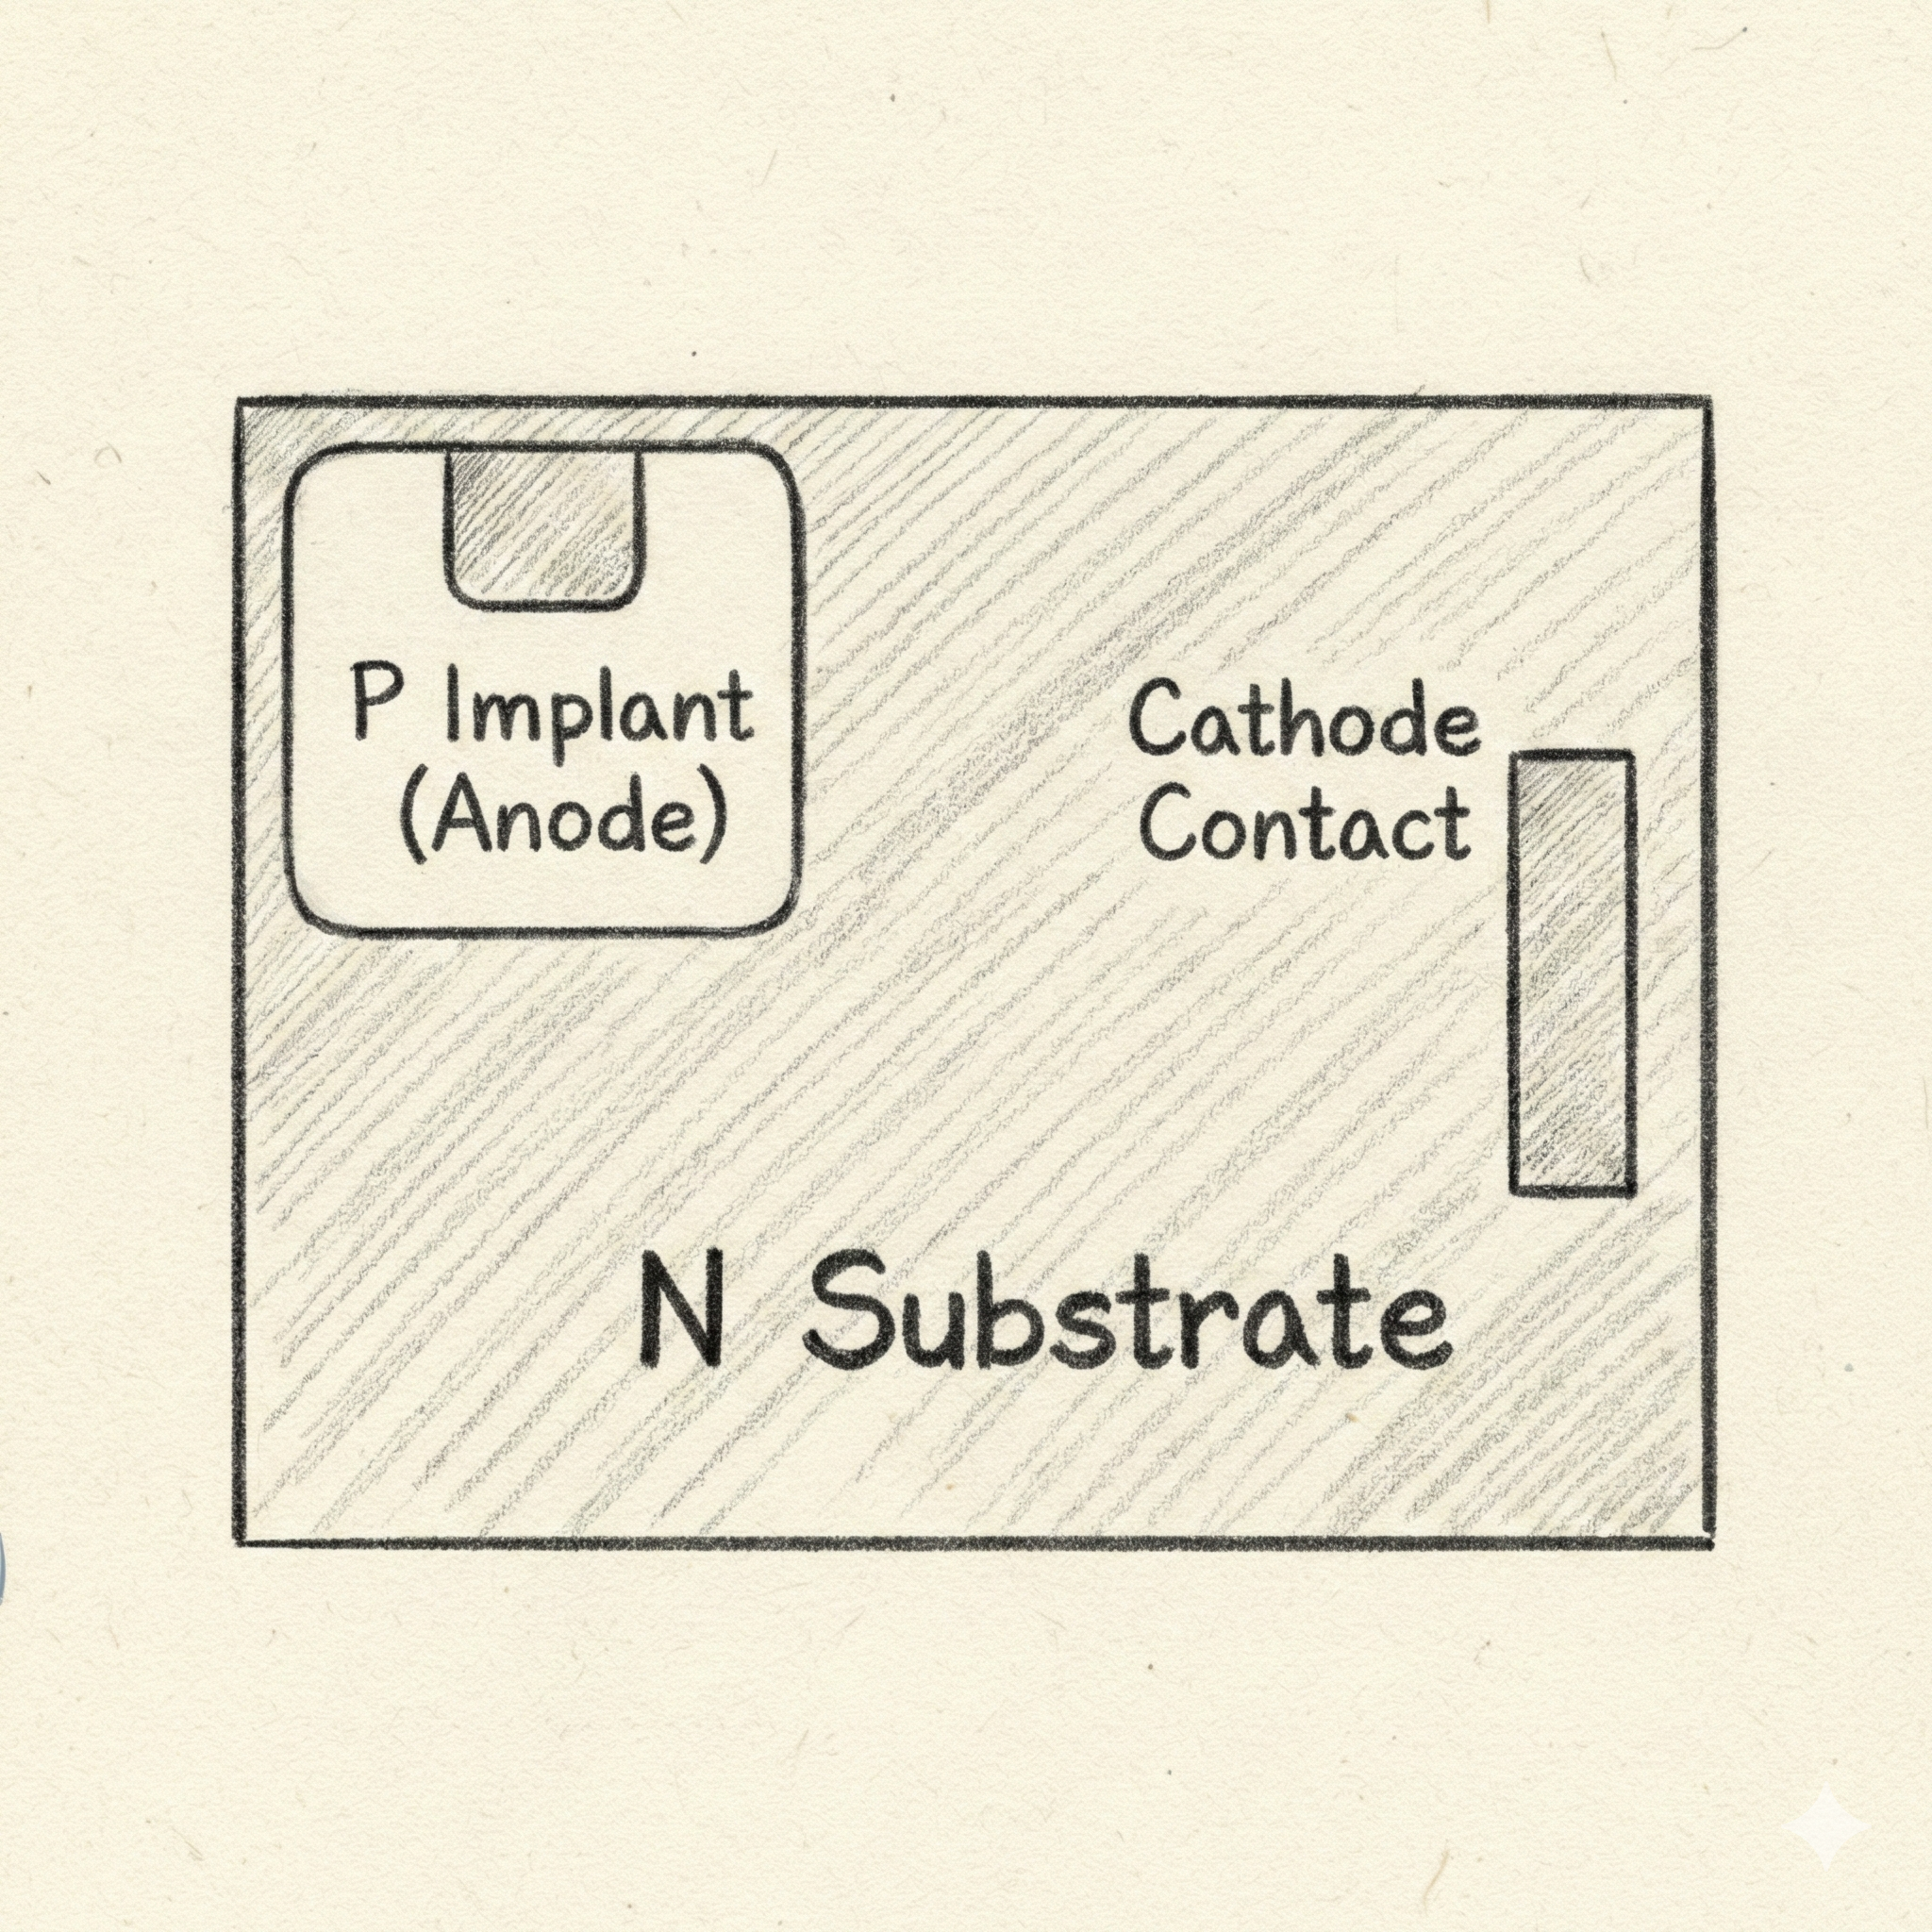
\includegraphics[width=\linewidth]{PD_sketch_top.png}\\[-0.5mm]
  {\scriptsize Top view (layout)}
\end{minipage}

\end{frame}

\begin{frame}{Experiments | Semiconductor example}
\small
\textbf{Context.}
We consider a steady-state concentration $y$ of a species in a bounded domain $\Omega \subset \mathbb{R}^2$
(with $y=0$ on $\partial\Omega$). Species are \emph{generated} in a localized subregion and can be
\emph{removed} by placing sinks. We want the sinks to be \emph{spatially sparse}. This is a simplified description of a photodiode in steady-state operation

\medskip
\textbf{State equation (diffusion).}
With diffusion coefficient $D>0$ and operator
\[
A_D := -D\Delta,\qquad y|_{\partial\Omega}=0,
\]
the steady-state balance reads
\[
A_D y \;=\; g - u \quad \text{in }\Omega,
\]
where $g$ is a prescribed generation term (here: constant on a small central square, $0$ outside)
and $u$ is the sink control.

\medskip
\textbf{Optimal control problem (measure-sparse control).}
We set the desired target to $z\equiv 0$ (remove species everywhere) and penalize the sink by a
\emph{measure norm} to promote sparsity:
\[
\min_{u\in \mathcal{M}(\Omega)}\;
\frac12\|y(u)-z\|_{L^2(\Omega)}^2 \;+\; \alpha \|u\|_{\mathcal{M}(\Omega)}
\qquad\text{s.t.}\qquad
A_D y = g-u,\; y|_{\partial\Omega}=0.
\]
Here $\alpha>0$ controls the sparsity strength: larger $\alpha$ yields fewer/stronger sink locations.
\end{frame}

\begin{frame}{Experiments | Semiconductor example}
    
\small

\textit{Numerical solution on $\Omega=[-1,1]^2$ (Dirichlet BC)}

\vspace{0.3em}
\includegraphics[width=\linewidth]{result_semic_4.png}

\parbox{\linewidth}{For low diffusitivity the optimized sink $u$ concentrates on pointlike structures surrounding the generation region. In contrast, in higher diffusivity environments, a ring like structure appears similar like a net for collecting the carriers. This structure is a direct consequence of the measure penalty, which promotes sparsity by
localizing the control on sets of small measure.}
\end{frame}

% ============================================================
% 17. ALTERNATIVE ROUTE: FEM SEQUEL IDEA
% ============================================================
\begin{frame}{Alternative numerical route: variational discretization (FEM sequel)}
\begin{block}{Different philosophy}
Discretize only the \emph{state} equation by FEM, keep $u\in\M(\Om)$ continuous.
\end{block}

\begin{block}{Key theorem (informal)}
The discrete optimizer can be chosen as a \emph{finite combination of Diracs at mesh nodes}:
\[
u_h^\ast = \sum_{j=1}^{N(h)} \lambda_j \delta_{x_j}.
\]
\end{block}

\begin{alertblock}{Comparison}
\begin{itemize}
  \item Predual approach: smooth variable + box constraints + Newton
  \item FEM sequel: state discretization induces nodal sparsity automatically
\end{itemize}
\end{alertblock}
\end{frame}

% ============================================================
% 18. CONCLUSION
% ============================================================
\begin{frame}{Conclusion}
\begin{block}{Main messages}
\begin{itemize}
  \item Measure controls model localized actuation and yield sparse optimal solutions
  \item Very weak solutions provide well-posed PDE state equations for $u\in\M(\Om)$
  \item Fenchel duality gives a predual Hilbert-space formulation with $\norm{p}_\infty\le \alpha$
  \item KKT structure explains sparsity: $u^\ast$ lives on the active set $\{|p^\ast|=\alpha\}$ 
\end{itemize}
\end{block}

\begin{alertblock}{Takeaway}
Predual reformulation turns a difficult nonsmooth measure problem into a numerically friendly box-constrained PDE problem.
\end{alertblock}

\bigskip
\centering
\textbf{Thank you!}
\end{frame}

\end{document}
